\section{Laboratory work implementation}

\subsection{Tasks and Points}

În cadrul lucrării au fost realizate următoarele funcționalități ale calculatorului:
\begin{itemize}
\item[•] operațiil +, -, /, *;
\item[•] operațiile  putere, radical, InversareSemn(+/-);
\item[•] operații cu numere zecimale;
\item[•] divizare proiectului în doua module - Interfața grafică(Modul GUI) și Modulul de bază(Core Module).

\end{itemize}

\end{enumerate}

\subsection{Analiza lucrarii de laborator}

	În cadrul acestei lucrări de laborator, a fost înaintată ca cerință de bază crearea unui calculator folosind interfață grafică. Limbajul ales pentru realizarea acestui proiect este C#, deoarece oferă posibilități mari de creare a interfețelor și este ușor de înușit. IDE-ul utilizat este Visual Studio.
	Inițial am creat interfața calculatorului, utilizând elementele grafice prestabilite de limbaj cu amplasarea butoanelor și chenarelor necesare. Ulterior, am modificat setările implicite ale elementelor, personalizându-le. 
	Interfața conține:
	\begin{itemize}
	\item 21 de butoane active;
	\item un textbox unde apare informația tastată pe butoane.
	\end{itemize}
	
	\textbf{Butonul "+"}
	
	   private void plusButton_Click(object sender, EventArgs e)
	   
        {
        
            number01 = float.Parse(numbersTextBox.Text);
            
            numbersTextBox.Text = "";
            
            plusButtonCounter++;
            
        }
	
	\textbf{Butonul "="}
	
	private void equalButton_Click(object sender, EventArgs e)
        
        {
            number02 = float.Parse(numbersTextBox.Text);
            
            if (plusButtonCounter == 1)
            
            { 
                numbersTextBox.Text = "" + (number01 + number02);
                
                plusButtonCounter = 0;
                
            }
           
            else if (minusButtonCounter == 1)
            {
                
                numbersTextBox.Text = "" + (number01 - number02);
               
                minusButtonCounter = 0;
                
            }
            
            else if (multiplyButtonCounter == 1)
            
            {
               
                numbersTextBox.Text = "" + (number01 * number02);
               
                multiplyButtonCounter = 0;
                
            }
            
            else if (divideButtonCounter == 1)
            
            {
                
                if (number02 == 0)
                
                {
                    
                    MessageBox.Show("Nu se admite impartirea la 0!");
                    
                }
                
                else
                
                {
                    
                    numbersTextBox.Text = "" + (number01 / number02);
                  
                    divideButtonCounter = 0;
                }
            }
        }
   
   \textbf{Butonul "C"}
   
  private void clearButton_Click(object sender, EventArgs e)
        
        {
           
            numbersTextBox.Text = numbersTextBox.Text.Substring(0, numbersTextBox.Text.Length - 1);
       
        }

        private void clearenterButton_Click(object sender, EventArgs e)
        
        {
            
            numbersTextBox.Text = "";
            
        }
   

    
\subsection{Imagini}

\begin{figure}[!ht]
\centering
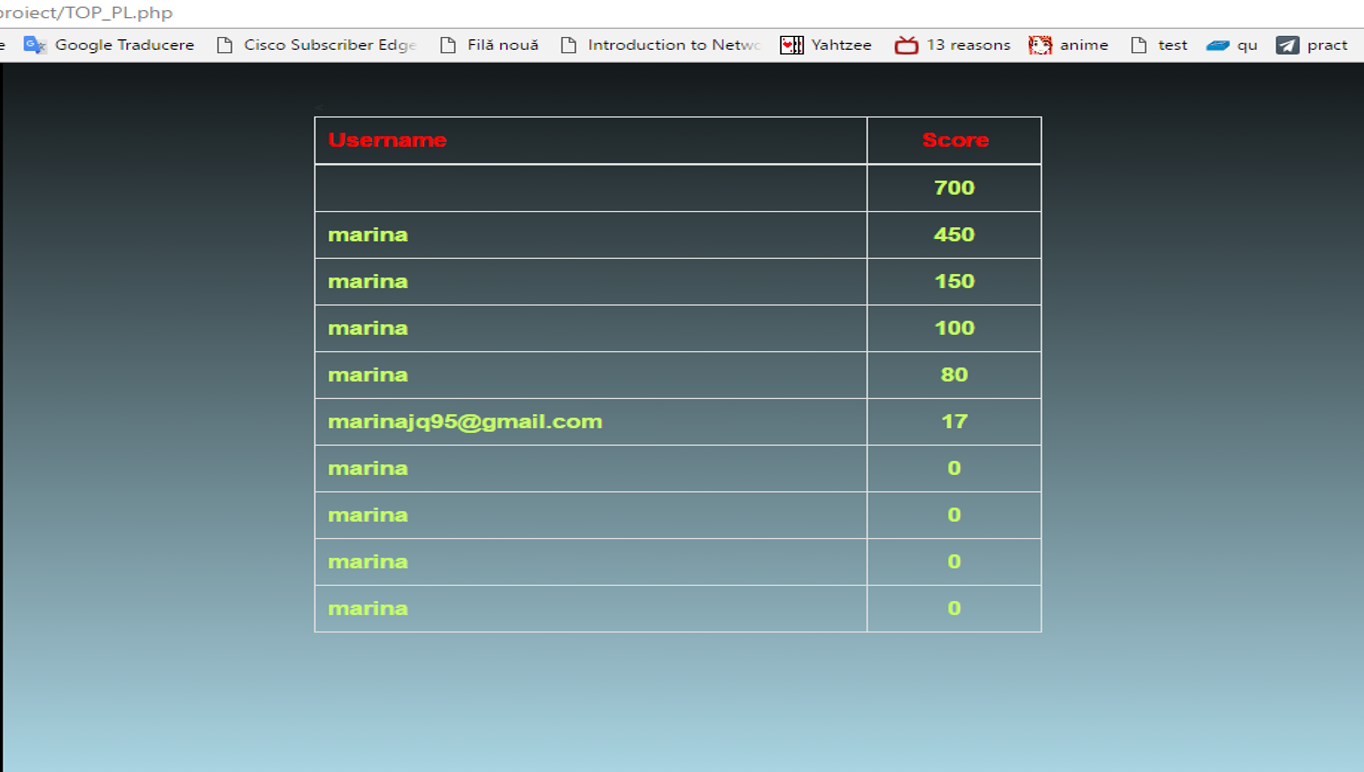
\includegraphics[width=0.3\textwidth]{1}
\caption{Interfața calculatorului, \cite{ImRef}}
\label{Im_label}
\end{figure}

\begin{figure}[!ht]
\centering

\includegraphics[width=0.3\textwidth]{2}
\caption{Radical din 52, \cite{ImRef}}
\label{Im_label}
\end{figure}

\begin{figure}[!ht]
\centering
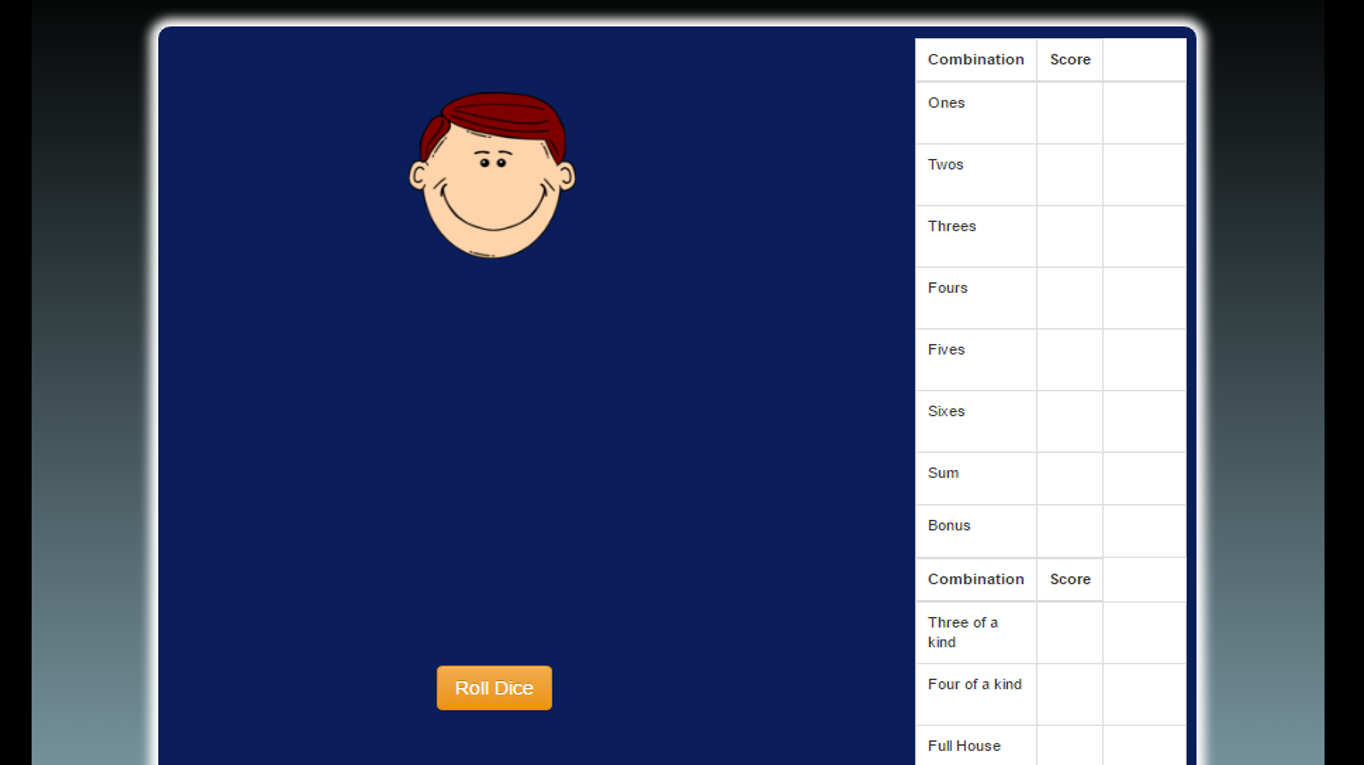
\includegraphics[width=0.3\textwidth]{3}
\caption{Patratul lui 14,23 \cite{ImRef}}
\label{Im_label}
\end{figure}


\begin{figure}[!ht]
\centering

\includegraphics[width=0.3\textwidth]{4}
\caption{Utilitatea butonului C \cite{ImRef}}
\label{Im_label}
\end{figure}

\clearpage